\documentclass[12pt]{article}

\usepackage[utf8x]{inputenc} % Включаем поддержку UTF8  
\usepackage[russian]{babel}  % Включаем пакет для поддержки русского языка  
\usepackage{hyperref}        % Для гиперссылок

% Математика
\usepackage{amsmath,amsfonts,amssymb,amsthm,mathtools} % AMS
\usepackage{icomma}
\usepackage{mathrsfs}

\usepackage{xcolor}

% Прога
\usepackage{etoolbox}
\usepackage{listings}

\definecolor{codegreen}{rgb}{0,0.6,0}
\definecolor{codegray}{rgb}{0.5,0.5,0.5}
\definecolor{codepurple}{rgb}{0.58,0,0.82}
\definecolor{backcolour}{rgb}{0.95,0.95,0.92}

\lstdefinestyle{mystyle}{
	backgroundcolor=\color{backcolour},   
	commentstyle=\color{codegreen},
	keywordstyle=\color{magenta},
	numberstyle=\tiny\color{codegray},
	stringstyle=\color{codepurple},
	basicstyle=\ttfamily\footnotesize,
	breakatwhitespace=false,         
	breaklines=true,                 
	captionpos=b,                    
	keepspaces=true,                 
	numbers=left,                    
	numbersep=5pt,                  
	showspaces=false,                
	showstringspaces=false,
	showtabs=false,                  
	tabsize=2
}

\lstset{style=mystyle}

% Цвета
\usepackage{xcolor}

% Картинки
\usepackage{graphicx}
\graphicspath{ {./images/} }

\usepackage{tikzsymbols}

% Работа с таблицами
\usepackage{array,tabularx,tabulary,booktabs} % Дополнительная работа с таблицами
\usepackage{longtable}  % Длинные таблицы
\usepackage{multirow} % Слияние строк в таблице

% Нумерованные списки
\usepackage[shortlabels]{enumitem} % Разные лейблы

% Текст
\usepackage[normalem]{ulem}  % для зачеркивания текста

\newtheorem{property}{Свойство}
\newtheorem{consequence}{Следствие}[property]

\begin{document}
	
	\thispagestyle{empty}
	\begin{center}
		\textbf{ПРАВИТЕЛЬСТВО РОССИЙСКОЙ ФЕДЕРАЦИИ}
		
		\vspace{5ex}
		
		\textbf{Федеральное государственное автономное образовательное учреждение \\ высшего образования \\ <<Национальный исследовательский университет \\ <<Высшая школа экономики>>}
	\end{center}
	\vspace{5ex}
	
	\begin{center}
		Московский институт электроники и математики им. А.Н. Тихонова  
		
		\vspace{5ex}
		
		Департамент прикладной математики
		
		\vspace{10ex}
		\textbf{Отчёт \\ по лабораторной работе A3 \\ по курсу <<Компьютерный практикум>> \\ Задание № 13}
		\vspace{7ex}
		
	\end{center}
	
	\begin{center} 
		\begin{tabular}{| p{0.3\linewidth}| p{0.3\linewidth}| p{0.3\linewidth}|}
			\hline	
			ФИО студента & Номер группы & Дата \\  \hline
			& & \\  
			Кейер Александр \newline Петрович & БПМ-231 & \today \\  
			& & \\  \hline		
		\end{tabular}
	\end{center}
	
	\begin{center}
		\vspace{3ex}
		
		\vfill
		
		\normalsize
		
		\textbf{Москва, 2023}
	\end{center}
	
	\newpage
	
	%---------------------------------------------------------------------------------
	
	\section*{Задание}
	
	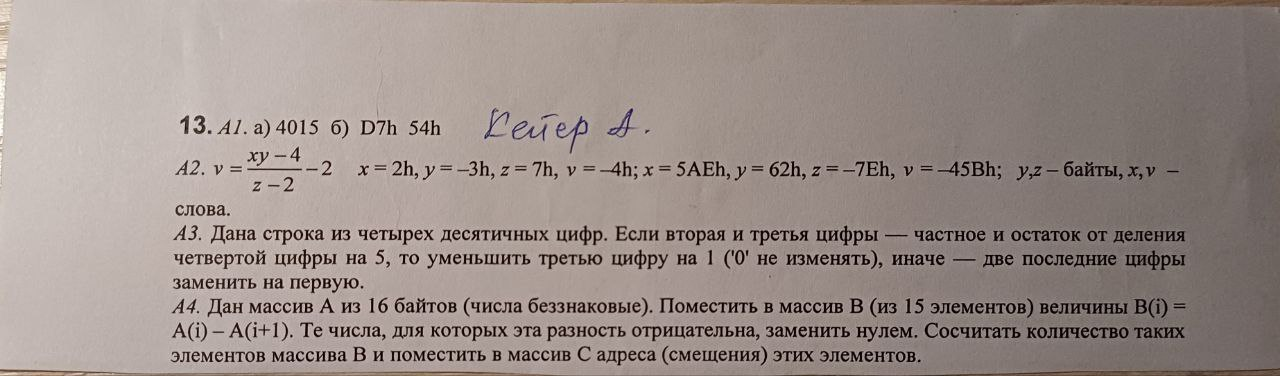
\includegraphics[width=400pt]{variant_13.jpg}
	
	Дана строка из четырех десятичных цифр. Если вторая и третья цифры -- частное и остаток от деления четвертой цифры на 5, то уменьшить третью цифру на 1 ('0' не изменять), иначе -- две последние цифры заменить на первую.
	
	\newpage
	
	%---------------------------------------------------------------------------------
	
	\section*{Решение}\addcontentsline{toc}{section}{}
	
	\begin{lstlisting}[language=C]
	#include <stdio.h> // Input/output library.
	#include <string.h> // String library for special function: strlen etc.
	
	#define sLength 5
	
	int testCounter = 1;
	
	// Function validating string.
	int isSValid(char s[sLength]) {
		
		// Check string length.
		if (strlen(s) < 4) {
			return 0;
		}
		
		// Check string symbols.
		for (int i = 0; s[i] != '\0'; i++) {
			if (s[i] > '9' || s[i] < '0') {
				return 0;
			}
		}
		
		return 1;
	}
	
	void test(char s[sLength]) {
		printf("Test %d.\n", testCounter++);
		printf("Entered string: %s\n", s);
		
		// Validating string.
		if (!isSValid(s)) {
			printf("The string should contain only decimal digits and conatain 4 symbols.\n");
			printf("\n===========\n\n");
			return;
		}
		
		s[0] -= '0';
		s[1] -= '0';
		s[2] -= '0';
		s[3] -= '0';
		
		// Asembly insertion.
		__asm__(
		"mov al, %3         # s[3] --> al \n"
		"cbw                # s[3] --> word \n"
		"mov bl, 5          # 5 --> bl \n"
		"div bl             # ax / bl \n"
		
		"cmp al, %1         # s[1] --> al \n"
		"jne REPLACE        # jump to REPLACE \n"
		
		"cmp ah, %2         # s[2] --> ah \n"
		"jne REPLACE        # jump to REPLACE \n"
		
		"cmp ah, 0          # ah == 0 \n"
		"je EXIT            # jump to EXIT \n"
		
		"dec ah             # ah-- \n"
		"mov %2, ah         # ah --> s[2] \n"
		"jmp EXIT           # jump to EXIT \n"
		
		"REPLACE: \n"
		"mov bl, %0         # s[0] --> bl \n"
		"mov %2, bl         # bl --> s[2] \n"
		"mov %3, bl         # bl --> s[3] \n"
		
		"EXIT: \n"
		"nop"
		:     
		: "m" (s[0]), "m" (s[1]), "m" (s[2]), "m" (s[3]) 
		: "%eax", "%ebx"
		);
		
		s[0] += '0';
		s[1] += '0';
		s[2] += '0';
		s[3] += '0';
		
		printf("Answer: %s\n", s);
		printf("\n===========\n\n");
	}
	
	int main() {
		// Test 1.
		char s1[sLength] = "2149";
		test(s1);
		
		// Test 2.
		char s2[sLength] = "2105";
		test(s2);
		
		// Test 3.
		char s3[sLength] = "2106";
		test(s3);
		
		// Test 4.
		char s4[sLength] = "2016";
		test(s4);
		
		// Test 5.
		char s5[sLength] = "216";
		test(s5);
		
		// Test 6.
		char s6[sLength] = "av123";
		test(s6);
		
		// User test.
		char s[sLength];
		printf("Please, enter string of four decimal digits without spaces: ");
		fgets(s, sLength + 1, stdin);
		s[strlen(s) - 1] = '\0';
		test(s);
		
		return 0;
	}
	\end{lstlisting}
	
	\newpage
	
	%---------------------------------------------------------------------------------
	
	\section*{Тесты}\addcontentsline{toc}{section}{}
	
	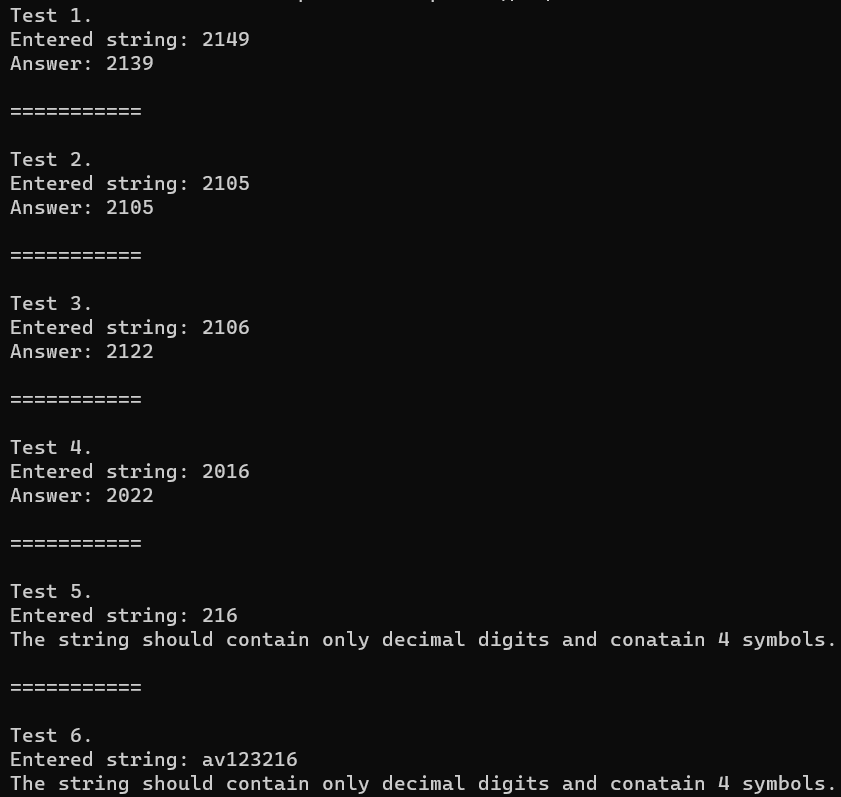
\includegraphics[width=400pt]{tests.png}
	
\end{document}
